\documentclass[border=10pt]{standalone}
\usepackage{tikz}
\usetikzlibrary{positioning,fit,arrows.meta,calc}

\begin{document}
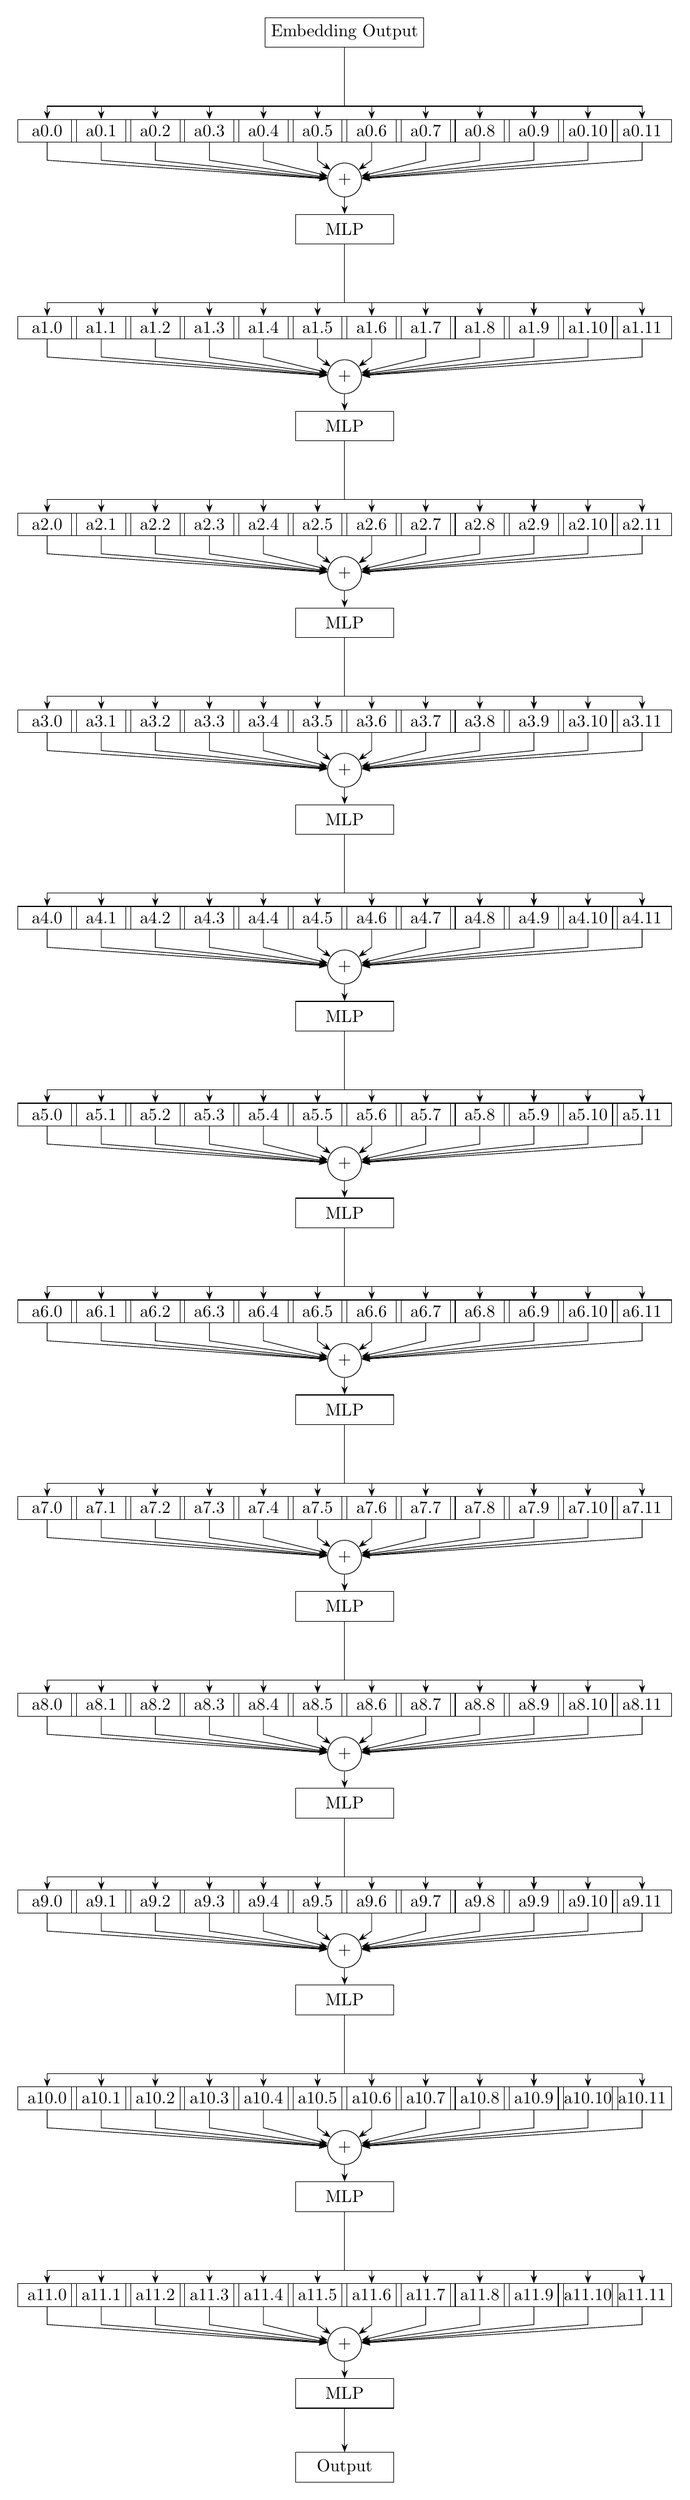
\begin{tikzpicture}[
    box/.style={rectangle,draw,minimum width=2cm,minimum height=0.6cm},
    attention/.style={rectangle,draw,minimum width=1.2cm,minimum height=0.4cm},
    layer/.style={rectangle,draw,dashed,inner sep=0.3cm},
    arrow/.style={-Stealth}
]

\def \LAYERHEIGHT {4.0}; % height of a layer

% Input
\node[box] (input) at (0,0) {Embedding Output};

% Define a style for attention head column
\foreach \l in {0,...,11} {
    % Layer label and box
    % \node[layer,below=0.8cm of input.south] (layer\l) {};
    % \node[left] at (layer\l.west) {Layer \l};
    \pgfmathsetmacro \lPrevious {int(\l - 1)}
    % Attention heads
    \foreach \h in {0,...,11} {
        \node[attention] (a\l\h) at ($(-6.05+\h*1.1,-2-\l*\LAYERHEIGHT)$) {a\l.\h};
        \ifnum \l > 0
            \draw[arrow] (mlp\lPrevious) -- ($(mlp\lPrevious)-(0,1.5)$) -- ($(mlp\lPrevious)-(6.05-\h*1.1,1.5)$) -- (a\l\h);
        \fi
    }

    % Connect previous layer's MLP to current layer attention heads
    
    
    % Concatenation and MLP for each layer
    \node[circle,draw] (concat\l) at (0,-3-\l*\LAYERHEIGHT) {+};
    \node[box] (mlp\l) at (0,-4-\l*\LAYERHEIGHT) {MLP};
    
    % Connect attention heads to concat
    \foreach \h in {0,...,11} {
        \draw[arrow] (a\l\h) -- ($(concat\l)+(-6.05+\h*1.1,0.4)$) -- (concat\l);
    }
    
    % Connect concat to MLP
    \draw[arrow] (concat\l) -- (mlp\l);
    
    % % Connect to next layer or output
    % \ifnum\l<12
    %     \draw[arrow] (mlp\l) -- ($(mlp\l)+(0,-0.3)$); -> IS HOW YOU CAN CALL THE COORDINATES OF AN ALREADY DRAWN NODE (basically math inside the tikz env.
    % \fi
}

% Connect input to first layer
\foreach \h in {0,...,11} {
    \draw[arrow] (input) -- ($(input)-(0,1.5)$) -- ($(input)-(6.05-\h*1.1,1.5)$) -- (a0\h);
}


% Output
\node[box] (output) at (0,-5.5-11*\LAYERHEIGHT) {Output};
\draw[arrow] (mlp11) -- (output);

\end{tikzpicture}
\end{document}